% !TeX spellcheck = en_GB
% /*
%  * ----------------------------------------------------------------------------
%  * "THE BEER-WARE LICENSE" (Revision 42):
%  * <michi.wieland@hotmail.com> wrote this file. As long as you retain this notice you
%  * can do whatever you want with this stuff. If we meet some day, and you think
%  * this stuff is worth it, you can buy me a beer in return. Michael Wieland
%  * ----------------------------------------------------------------------------
%  */

\documentclass[
a4paper,
oneside,
10pt,
fleqn,
headsepline,
toc=listofnumbered, 
bibliography=totocnumbered]{scrartcl}

% deutsche Trennmuster etc.
\usepackage[T1]{fontenc}
\usepackage[utf8]{inputenc}
\usepackage[english, ngerman]{babel} % \selectlanguage{english} if  needed
\usepackage{lmodern} % use modern latin fonts

% Custom commands
\newcommand{\AUTHOR}{Fabian Hauser \& Muriele Trentini}
\newcommand{\INSTITUTE}{Hochschule für Technik Rapperswil}
\newcommand{\GITHUB}{https://github.com/michiwieland/hsr-zusammenfassungen}
\newcommand{\LICENSEURL}{https://en.wikipedia.org/wiki/Beerware}
\newcommand{\LICENSE}{
"THE BEER-WARE LICENSE" (Revision 42):
<michi.wieland@hotmail.com> wrote this file. As long as you retain this notice you
can do whatever you want with this stuff. If we meet some day, and you think
this stuff is worth it, you can buy me a beer in return. Michael Wieland	
}

% Jede Überschrift 1 auf neuer Seite
\let\stdsection\section
\renewcommand\section{\clearpage\stdsection}

% Multiple Authors
\usepackage{authblk}

% Layout / Seitenränder
\usepackage{geometry}

% Inhaltsverzeichnis
\usepackage{makeidx} 
\makeindex

\usepackage{url}
\usepackage[pdfborder={0 0 0}]{hyperref}
\usepackage[all]{hypcap}
\usepackage{hyperxmp} % for license metadata

% Glossar und Abkürzungsverzeichnis
\usepackage[acronym,toc,nopostdot]{glossaries}
\glossarystyle{altlisthypergroup}
\usepackage{xparse}
\DeclareDocumentCommand{\newdualentry}{ O{} O{} m m m m } {
	\newglossaryentry{gls-#3}{name={#5},text={#5\glsadd{#3}},
		description={#6},#1
	}
	\makeglossaries
	\newacronym[see={[Siehe:]{gls-#3}},#2]{#3}{#4}{#5\glsadd{gls-#3}}
}
\makeglossaries

% Mathematik
\usepackage{amsmath}
\usepackage{amssymb}
\usepackage{amsfonts}
\usepackage{enumitem}

% Images
\usepackage{graphicx}
\graphicspath{{images/}} % default paths

% Boxes
\usepackage{fancybox}

%Tables
\usepackage{tabu}
\usepackage{booktabs} % toprule, midrule, bottomrule
\usepackage{array} % for matrix tables

% Multi Columns
\usepackage{multicol}

% Header and footer
\usepackage{scrlayer-scrpage}
\setkomafont{pagehead}{\normalfont}
\setkomafont{pagefoot}{\normalfont}
\automark*{section}
\clearpairofpagestyles
\ihead{\headmark}
\ohead{\AUTHOR}
\cfoot{\pagemark}

% Pseudocode
\usepackage{algorithm}
\usepackage{algorithmic}

% Code Listings
\usepackage{listings}
\usepackage{color}
\usepackage{beramono}

\definecolor{DarkPurple}{rgb}{0.4, 0.1, 0.4}
\definecolor{DarkCyan}{rgb}{0.0, 0.5, 0.4}
\definecolor{LightLime}{rgb}{0.3, 0.5, 0.4}
\definecolor{Blue}{rgb}{0.0, 0.0, 1.0}

\lstdefinestyle{eclipse-style}{
	language=Java,  
	columns=flexible,
	showstringspaces=false,     
	basicstyle=\footnotesize\ttfamily, 
	keywordstyle=\bfseries\color{DarkPurple},
	commentstyle=\color{LightLime},
	stringstyle=\color{Blue}, 
	escapeinside={£}{£}, % latex scope within code      
	morekeywords={length},
	numbers=left,
	numberstyle=\tiny\color{black},
	frame=single,
}
\lstset{style=eclipse-style}


% Theorems \begin{mytheo}{title}{label}
\usepackage{tcolorbox}
\tcbuselibrary{theorems}
\newtcbtheorem[number within=section]{definiton}{Definition}%
{fonttitle=\bfseries}{def}
\newtcbtheorem[number within=section]{remember}{Merke}%
{fonttitle=\bfseries}{rem}

% Template extensions
\newcommand\equalhat{\widehat{=}}
\newcommand\mathSpaceSeparator{\text{ }\text{ }\text{ }\text{ }}


% Dokumentinformationen
\newcommand{\SUBJECT}{Zusammenfassung}
\newcommand{\TITLE}{Programmieren und Formale Methoden}

\loadglsentries{glossar}

% pdf metadata
\hypersetup{
	pdfauthor={\AUTHOR},
	pdftitle={\SUBJECT \TITLE},
	pdfcopyright={\LICENSE},
	pdflicenseurl={\LICENSEURL}
}

\begin{document}
	
% Front page
\title{\TITLE}
\subject{\SUBJECT}
\author{\AUTHOR}
\affil{\INSTITUTE}
\date{\today}
\maketitle

\vfill

% Participate
\paragraph{Mitmachen} \hfill \\
Falls Du an diesem Dokument mitarbeiten willst, kannst Du das Dokument
auf GitHub unter \url{\GITHUB} forken.

% Licence
\paragraph{Lizenz} \hfill \\
\LICENSE

% Table of contents
\tableofcontents


% Glossar and acronyms (if included \loadglsentries{glossar})
\printglossary[type=\acronymtype]
\printglossary
\glsaddall


\section{Introduction}
The use of a formal language to describe and solve problems is central to computer science.

\begin{description}
	\item[Formal Methods] the application of theoretical computer science fundamentals. Motivation: use of mathematical analysis make computer programming more reliable and predictable.
	\item[Formal Language] Set of strings of symbols that are constrained by specific rules. Membership in this set can automatically be determined (mechanical processing possible)
	\item[Informal Language] Any living natural language
\end{description}

\section{Programming Paradigms}

Paradigm is a Worldview / Concept / Tought patterns.

OOP uses multiple of the paradigms below, but is not a paradigm in this sense.

\subsection{The Imperative Programming Paradigm}

Is imperative (de: Befehlend) and focuses on \emph{how} a program works, like a recipe. It uses commands to change the program's state.

A program (in this course) is a sequence of commands and the computation is a change of state.

Most hardware implementations of computer is imperative.

It is based on the Von Neumann architecture.

\subsubsection{Basic Building Blocks}

\begin{description}
	\item[Assignments (sate/store/heap)] x:= x+1 %TODO: COde
	\item[Sequential composition] ...; ...
	\item[Conditional excetion] if ... then ... else...
	\item[Repetition] while .. do .. / goto ...
\end{description}



\subsection{The Declarative Programming Paradigm}

Discribe logic of computation without expicitly describing its control flow.

\emph{What} should a programm accomplish, not how the language should do smth. (But it must still be computable in the end).

Programs are here theories of a formal logic. Computations are deductions.

Examples: Spreadsheets, Regex, Query Languages (SQL etc.), Functional programming languages (Haskel, ...), Logic programming (Prolog)

\subsubsection{The Functional Programming Paradigm}

Basis: The Lambda Calculus

Programs are function definitions, computations are function evaluations.

\subsubsection{The Logical Programming Paradigm}
Basis: Predicate logic

Programs are rules in predicate logic and computation is a proof of a predicate.



\section{Formal Proof (Propositional and Predicate logic)}

\begin{figure}
	\centering
	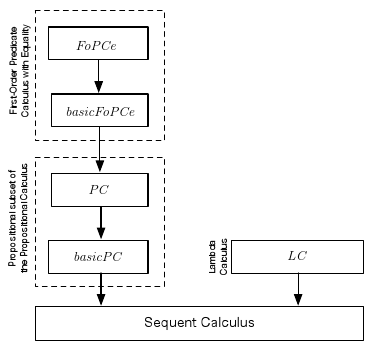
\includegraphics[width=0.7\linewidth]{images/sequent_calculus_overview}
	\caption{Overview calculus proof family.}
	\label{fig:sequentcalculusoverview}
\end{figure}

\subsection{refresher ''Diskrete Mathematik''}
Kinds of logic: Boolean, ''Aussagenlogik'' ($\Rightarrow, \Leftrightarrow, \wedge, \vee, \neg$), ''Prädikatenlogik'' ($\forall,\exists, R(x)$)

Proofs: by induction, direct, indirect, by contradiction

\subsection{What are formal and informal proofs?}
In an \emph{informal proof} arguments are presented as explanations in natural language (like most mathematical textbooks; needs a human to check correctness)

A \emph{formal proof} is constructed using well-formed formulas of a formal language and formally defined rules of inference.
 They can be checked by a machine and sometimes be mechanically constructed. Computer programs are able to assist proving (e.g. like Excel), sometimes a proof is even not practically possible without them.

\subsection{Sequent Calculus style}

The sequent calculus style is widely used in computer science, for instance to define program semantics or typing rules.

\subsection{Sequent Calculus}
A sequent is a generic name for a statement that we want to prove.
\subsubsection{Proof Rules}

 A device to construct proofs.
 
 \[
 \frac{\overrightarrow{A}}{C} \boldsymbol{r}
 \]
 
 \begin{description}
	 	\item[$r$] Rule name
	 	\item[$C$] Consequent (to be proven)
	 	\item[$\vec{A}$] Antecedents: list of sequents (vector).
 	\end{description}
 	
 
 We want to proof $C$ out of multiple sequent proof rules $A_1, A_2, ..., A_n$ with the rule $r$. If there is no $A$ above the line, the proof rule is an axiom. The order of proof rules in $A$ is important and not permutable.
 
 To build a complete proof, all proof rules must be proven up to an axiom.


\subsubsection{Definitions}

\begin{description}
	\item[Sequent] a generic name for a statement that
we want to prove.
	\item[Proof Rule] A rule $r$ to proof a consequent $C$ with sequents in $A$
	\item[pending sub-goal] A sequent which is not yet proven by an axiom.
	\item[Axiom] Proof rule without sequent $A$; basic element assumed to be true. \\
	There should be as few axioms as possible.
	\item[Calculus (or Theory)] (possibly infinite) set of proof rules $r_1$, $r_2$.
	\item[Proof (or Derivations)] Ordered proof rules in a tree, so that all proof rules are proven by an axiom.
	\item[incomplete Proof] has at least one pending subgoal
\end{description}

\subsubsection{Example}

\paragraph{Type checking proof}

of the shorthand if else construct for integers.

\[
	\frac{
			\frac{
				\frac{}{x::int}x_{int} \text{   } \frac{}{y::int}y_{int}
			}{(x > y)::bool}>_{int} \text{   }
		  \frac{
				\frac{}{x::int}x_{int} \text{   } \frac{}{y::int}y_{int}
			}{(x - y)::int} -_{int1} \text{   }
			\frac{
				\frac{}{y::int}y_{int} \text{   } \frac{}{x::int}x_{int}
			}{(y - x)::int} -_{int2}
		}{(x>y? x - y : y - x)::int} condExpr_{int}
\]

\subsection{Propositional Calculus (DE: Aussagenlogik)}

Example:\\*
If it is raining then it is cloudy.\\*
It is raining.\\*
Therefore it is cloudy.

\subsubsection{Definitions}
\begin{description}
	\item[Predicate] Truth value that we can assume or wish to prove (also called proposition).
	\item[Sequent] $H \vdash G$, read: Under the hypotheses $H$, prove the goal $G$ \hfill \\
	\begin{description}
		\item[$H$] Hypoteheses: a (finite) set of predicates
		\item[$\vdash$] therefore/entails
		\item[$G$] Goal: a single predicate
	\end{description}
\end{description}

\subsubsection{basicPC: Basic Propositional Calculus}

The basicPC syntax is the minimal subset required to write propositional logic. The syntax is defined in BNF (Bacus-Naur-Form).

\[
	P ::= \bot | \neg P | P \land P | P
\]

The rules above are a logical \emph{NAND}, which are also the most basic element of electronical circuits.

\subsubsection{Proof Rule Schema}

Proof Rule schemas represent an infinite number of proof rules of the same form. They use ''meta variables'', that can be instantiated (that is, replaced).

\paragraph{Example} 
\[
	\frac{
		\text{H} \vdash P \mathSpaceSeparator \text{H}, P \vdash C
	 }{
		\text{H} \vdash Q
	} cut
\]

In this example, H, $P$ and $Q$ are meta-variables that need to be initiated with concrete predicates, e.g. $A$, $B$ and $C$: \begin{align*}
  \text{H} &:= \{A\} \\
	P &:= B \\
	Q &:= C \\
\end{align*}

Commas, like in the example $\text{H}, P \vdash C$, are used to create a new set containing alle elements from H and $P$.

\subsubsection{Proof Rules of basicPC}

\begin{align*}
	  \frac{}{H,P \vdash P}
	& hyp
	& \text{If P is in hypothesis and goal the sequent is proven} \\
		\frac{H \vdash Q}{\text{H},P \vdash Q}
	& mon
	& \text{We can leave out individual Hypotheses} \\
	  \frac{H \vdash P \mathSpaceSeparator H, P \vdash Q}{H \vdash Q}
	& cut
	& \text{Allows you to introduce lemmas to simplify proving } H \vdash Q \\
	\frac{}{H, \bot \vdash P}
	& \bot hyp
	& \text{With an inconsistent system, you are able to prove anything.} \\
	\frac{H, \neg P \vdash \bot}{H \vdash P}
	& contr
	& \text{Proof by contradiction: If we assume P is false, our hypotheses are inconsistent.} \\
	\frac{H, P \vdash \bot}{H \vdash \neg P}
	& \neg goal
	& \text{negations can “jump” over turnstyle} \\
	\frac{H \vdash P}{H, \neg P \vdash Q}
	& \neg hyp
	& \text{negations can “jump” over turnstyle} \\
	\frac{H \vdash P \mathSpaceSeparator H \vdash Q}{H \vdash P \land Q}
	& \land goal
	& \text{If we want to prove } P \land Q \text{ , we can prove } P \text{ and } Q \text{ separately.} \\
	\frac{H,P,Q \vdash R}{H,P \land Q \vdash R}
	& \land hyp
	&	\text{If we have a conjunction in Hypothesis, we can assume the Hypotheses seperatly}
\end{align*}

\subsubsection{Operators}

The $\equalhat$-Sign denotes a syntactic equivalence.

\begin{align*}
	\top & \equalhat \neg \bot 
	& \text{( $\equalhat_{\top}$)} \\
	P \lor Q & \equalhat \neg(\neg P \land \neg Q)
	& \text{( $\equalhat_{\lor}$)} \\
	P \Rightarrow Q & \equalhat \neg P \lor Q
	& \text{( $\equalhat_{\Rightarrow}$)} \\
	P \Leftrightarrow Q & \equalhat (P\Rightarrow Q) \land (Q \Rightarrow R)
	& \text{( $\equalhat_{\Leftrightarrow}$)} \\
\end{align*}

\emph{Important}: Both proof rules and syntactic rewriting can be used in a single proof!

\subsubsection{Additional Proof Rules}

Additional proof rules for operators: %TODO: Slide 12


\subsection{First order Predicate Calculus}

We would like to extend predicate calculus PC to FoPCe via an intermediate step basicFoPCe to also allow Mathematical objects (numbers, functions, things, people etc.)

\subsubsection{Definition}

\begin{description}
	\item[FoPCe] first-order predicate calculus with equality
	\item[Expression] An expression is a formal statement denoting a mathematical object. Expressions cannot be proven. Examples: $f(x), x, g(x, f(x))$
	\item[Variables] A variable is an identifier that denotes an expression. It is just a place holder and may be a black box. Example: $x$
\end{description}

\subsubsection{Syntax}
\begin{align*}
	P &::= ...| \forall x.P | E = E | R(\vec{E}) 
	& \text{where R() and “=” are uninterpreted/special relationship symbols}\\
	E &::= x | f(\vec{E})
	& \text{where $\vec{E}$ is a List of Expressions}
\end{align*}	

\paragraph{Free and bound variables} \[
	\forall x .(f(x,y) = a \land A)
\]

$x$ is a bound variable: it is just a place holder. It's name has no significance and can be changed.

$y$ is a free variable that can be assigned ''externally''.

\subsubsection{Proof rules for basicFoPCe}

%TODO: slide 8 VL first order predicate calculus

\subsubsection{Excursion: Computation using FoPCe}
Example: We want to compute the reachability of nodes in a graph %TODO: evt graph zeichnen mit Tikz?

Step 1: Model the problem as a sequent in FoPCe \\

Nodes in a graph have a relationship \\
$R(x,y)$\qquad Denotes that node y can be reached from node x\\

We need a set of Hypotheses 'G' \\
Reflexive: $\forall x. R(x,x)$ \\
Transitiv: $\forall x.\forall y.\forall z. R(x,y) \land R(y,z) \Rightarrow R(x,z)$

Our specific Graph:\\
$R(a,b) \qquad R(b,c) \qquad R(c,d) \qquad R(p,q)$\\

Our Queries: \\
\begin{align*}
	&\text{Is node a reachable from node d:} &G &\vdash R(a,d)\\
	&\text{Which nodes are reachable from node a:} &G &\vdash \exists x.R(a,x)
\end{align*}

\subsubsection{Excursion: Equational Reasoning}
Equational reasoning is a different style of a formal proof \textbf{equivalent} to FoPCe Proofs. It is however specialized fpr proofs \emph{only involving equality}.
%TODO proof from slide 18 VL First order predicate Calculus

\section{Logic programming (Prolog)}
A Prolog program consists of a knowledge base (i.e. an intelligent database), which consists od rules and facts, and a query.
If you run the query, Prolog will answer with either “true” or “false”, depending on whether a proof could be found.
\subsection{First Prolog program}
We want to compute the validity of this syllogism: \\
All humans are mortal. \\
Socrates is human. \\
Therefore, Socrates is mortal.\\
Step 1: Model the argument as a sequent in FoPCe

\[
\text{H(x): x is human}\\
\text{M(x): x is mortal}\\
\text{s: Sokrates}\\
\forall x.H(x) \Rightarrow M(x),H(s) \vdash M(s)
\]

Step 2: Use Prolog to find a proof for the sequent

%TODO code slide 8/9 VL Logic programming Introduction

\section{Lambda calculus}

\section{Functional Programming (Haskell)}

\section{Multi-Paradigm Programming (Scala)}


\appendix

% Code Listings
\lstlistoflistings

% List of figures
\listoffigures

% List of tables
\listoftables

% Bibliography
\bibliographystyle{plain} 
\bibliography{literatur}

\end{document}
